\documentclass[12pt]{article}
\usepackage{amsmath}
\usepackage{amssymb}
\usepackage{graphicx}
\graphicspath{ {./images/} }
\begin{document}

Starting in calculus 3, we use 3d coordinate system rather than 2d.

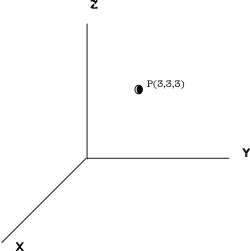
\includegraphics{3dgraph.png}

To form the graph, refer to the chart below.
\begin{quote}
	Point index to pinky finger in direction of 1; this shows the x-axis.
Then curl fingers towards 2 for the y-axis. The thumb indicates the z axis.	
\end{quote}

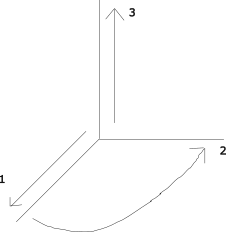
\includegraphics{howtomakegraph}

We use the \textbf{right hand rule} to get this (we use the right hand)\\
We can create a projection of a point onto xy, xz, yz plane by setting z, y, or x to 0. 

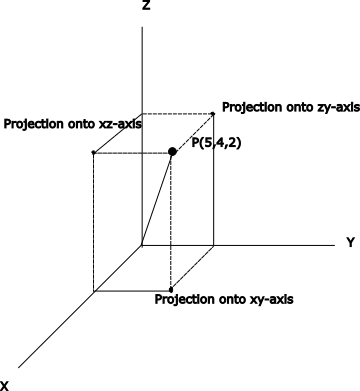
\includegraphics{projections-onto-3daxes}

Here the point P(5,4,2) is plotted and the projections onto the 3 planes are displayed.
From left to right: (0,4,2), (5,0,2), (5,4,0)

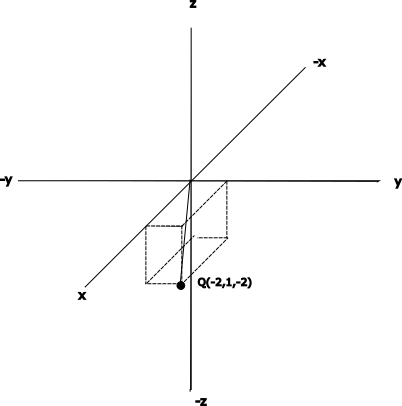
\includegraphics{projection2}

The graph above demonstrates a point Q(2,1,-2) where the x coordinates are now negative.
An error was made where the x coordinate in the graph is negative when it is in fact positive.

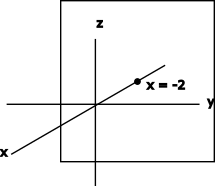
\includegraphics{parallelzy}
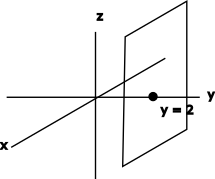
\includegraphics{parallelxz}

The preceding graphs demonstrate planes parallel to the zy and xz planes respectively. 
Notice for each of the graphs, there is a single fixed point and domains for unfixed coordinates are $\in{R}$.

Finally, below is a demonstration of a plane parallel to the xy plane.

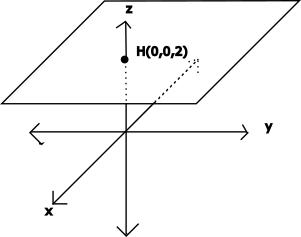
\includegraphics{parallelxy}

Below is a comparison between $x^2+y^2=1$, the equation for a circle, on a 2d graph vs on a 3d graph.

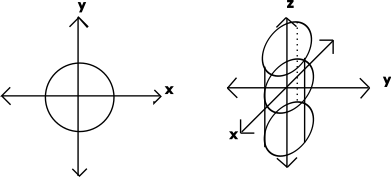
\includegraphics{circleequation}

\underline{Find distance from point A to point B}

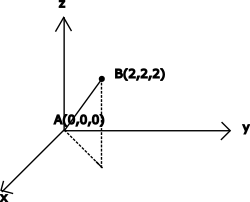
\includegraphics{distanceab}

Visualize: a triangle where you are finding hypotenuse, distance between point $A(0,0,0)$ and point $B(0,0,0)$, otherwise known as the magnitude of $\vec{AB}$, which can be represented as $|\vec{AB}|$.

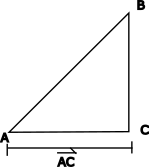
\includegraphics{distanceab-2d}

We can find $|\vec{AC}|$ by taking the result of applying pythagorean function on difference between the X and Y coordinates on the points B and A.
\begin{flalign}
	Pythagoras = a^2+b^2=c^2\\
	a=x_b-x_a,\ b=y_b-y_a\\
	2^2+2^2=|\vec{AC}|^2\\
	\therefore{|\vec{AC}|=\sqrt{8}}
\end{flalign}.

Thus, we can solve for $|\vec{AB}|$ by then applying the pythagorean formula once more this time using $|\vec{AC}|$.  

\setcounter{equation}{0}
\begin{flalign}
	|\vec{AB}|=\sqrt{|\vec{AC}|^2+(z_b-z_a)^2}\\
	|\vec{AC}|^2=(x_b-x_a)^2+(y_b-y_a)^2=2^2+2^2\\
	|\vec{AB}|=\sqrt{2^2+2^2+2^2}\\
	\therefore{|\vec{AB}|=\sqrt{12}}
\end{flalign}.

As can be seen in (3), the equation for the distance between any given point $P(x,y,z)$ and the origin$(0,0,0)$ can be represented as:\\ $|\vec{P}|=\sqrt{x^2+y^2+z^2}$ 

We can also say that the distance between any 2 points $A(x_1,y_1,z_1)$ and $B(x_2,y_2,z_2)$ can be represented by the equation:\\
$|\vec{AB}|=\sqrt{(x_2-x_1)^2+(y_2-y_1)^2+(z_2-z_1)^2}$
 

Here is a sphere centered on point $R(h,k,l)$


\includegraphics{sphere}

The formula for a circle is $x^2+y^2=1$

Similarily, the formula for a sphere centered at the origin$(0,0,0)$ is: \\$x^2+y^2+z^2=1$

Standard form of a sphere:\\
$(x-h)^2+(y-k)^2+(z-l)^2=r^2$

...

Exercise: find the centre and radius of a sphere with equation:\\ $x^2+y^2+z^2+6x-4y-2z+6=0$

Group like terms.

\setcounter{equation}{0}
\begin{align}
	x^2+6x+y^2-4y+z^2-2z+6=0
\end{align}
Complete the square.
\begin{align}
	x^2+6x+9-9+y^2-4y+4-4+z^2-2z+1-1+6=0
\end{align}
Factor
\begin{align}
	(x+3)^2+(y-2)^2+(z-1)^2=8
\end{align}

Thus, the center of the sphere lies at coordinates $(-3,2,1)$ and the radius of the sphere is $\sqrt{8}$.
\end{document}
